\chapter{Objetivos, Alcance y Antecedentes}
\label{ch:objetivos_alcance_antecedentes}

En este capítulo se formalizan los fundamentos estratégicos, metodológicos y científicos sobre los cuales se erige la presente investigación. En primer lugar, se definen de manera unívoca el objetivo general y los objetivos específicos, asociándolos a hipótesis de éxito mensurables que guiarán la validación experimental del proyecto. Posteriormente, se delimita el alcance analítico e ingenieril del desarrollo ejecutado, explicitando tanto las inclusiones técnicas como las exclusiones impuestas por el estado de madurez de la tecnología cuántica actual. Finalmente, se expone un riguroso estado del arte que examina de forma crítica las limitaciones de los solucionadores exactos y heurísticos clásicos, contextualizando el surgimiento de los algoritmos variacionales híbridos y justificando técnicamente la elección del paradigma XY-QAOA frente a las alternativas tradicionales basadas en penalizaciones matemáticas.

\section{Objetivos del Proyecto (General y Específicos)}
\label{sec:objetivos_proyecto}

\subsection{Objetivo General}
El objetivo principal de este Trabajo de Fin de Máster consiste en diseñar, implementar, optimizar y evaluar de manera sistemática un algoritmo cuántico híbrido basado en el Algoritmo de Optimización Cuántica Aproximada (QAOA) para la resolución del problema de selección de carteras financieras sujeto a restricciones discretas duras de cardinalidad exacta ($K$). Dicho desarrollo se evalúa de manera crítica tanto en entornos de simulación numérica densa como frente a arquitecturas clásicas de referencia industrial.

\subsection{Objetivos Específicos}
Para asegurar la consecución del objetivo general, se desglosan los siguientes hitos específicos de carácter técnico e investigacional:
\begin{itemize}
    \item \textbf{OE1. Formulación y Modelado Matemático:} Mapear analíticamente la función de coste cuadrática del modelo de media-varianza de Markowitz y sus restricciones operativas hacia una estructura de Optimización Binaria Cuadrática No Restringida (QUBO) y, subsiguientemente, a un Hamiltoniano de Ising almacenable en registros de cúbits.
    \item \textbf{OE2. Diseño de Circuitos Avanzados con Preservación de Simetría:} Desarrollar e implementar en código cuántico un \textit{ansatz} variacional especializado basado en operadores de mezcla XY (\textit{XY-Mixer}) acoplados a la preparación de estados cuánticos de Dicke, con el fin de restringir físicamente la evolución del sistema dentro del subespacio factible.
    \item \textbf{OE3. Regularización Algorítmica de la Convergencia:} Diseñar e incorporar mecanismos de regularización matemática (incluyendo penalizaciones continuas de tipo Ridge $L_2$ y esquemas de evolución adiabática guiada) integrados en el bucle variacional clásica-cuántica para mitigar la problemática de los mínimos locales y optimizar la convergencia clásica.
    \item \textbf{OE4. Benchmarking Computacional Crítico:} Ejecutar una campaña exhaustiva de experimentos numéricos para comparar cuantitativamente el rendimiento del algoritmo desarrollado frente a solucionadores exactos clásicos (\textit{Gurobi Optimizer}) y metaheurísticas tradicionales (\textit{Simulated Annealing}), evaluando métricas clave como el \textit{Optimization GAP}, la tasa de viabilidad (\textit{feasibility}) y el coste temporal de cómputo.
\end{itemize}

\subsection{Hipótesis de Éxito}
El éxito científico y técnico de esta investigación se evalúa mediante los criterios de validación empírica formalizados en la Tabla \ref{tab:hipotesis_exito}.

\begin{table}[htbp]
    \centering
    \caption{Matriz de trazabilidad de objetivos específicos e hipótesis cuantitativas de éxito.}
    \label{tab:hipotesis_exito}
    \begin{tabular}{cp{5.5cm}p{6cm}}
        \toprule
        \textbf{Objetivo} & \textbf{Entregable / Indicador} & \textbf{Métrica de Éxito Cuantitativa} \\
        \midrule
        \textbf{OE1} & Formulación Ising válida. & Verificación analítica y equivalencia estricta de energías en espectro completo. \\
        \textbf{OE2} & Tasa de viabilidad del \textit{ansatz}. & Obtención de una viabilidad matemática intrínseca del $100\%$ en las muestras del circuito cuántico libre de ruido. \\
        \textbf{OE3} & Reducción de variabilidad en optimización clásica. & Disminución del número de evaluaciones de la CPU en un $\ge 15\%$ frente al bucle no regularizado. \\
        \textbf{OE4} & Rendimiento relativo frente a heurísticas clásicas. & Consecución de un \textit{Optimization GAP} medio $\le 5\%$ en instancias de tamaño NISQ intermedio ($N=14$). \\
        \bottomrule
    \end{tabular}
\end{table}

\section{Alcance y Delimitación del Estudio}
\label{sec:alcance_delimitacion}

\subsection{Fronteras del Proyecto e Inclusiones Técnicas}
El alcance de la solución de software desarrollada bajo el repositorio \texttt{etxaaniiz/tfm} contempla las siguientes dimensiones operativas de manera estricta:
\begin{enumerate}
    \item \textbf{Modelado Financiero:} Modelos de optimización aplicados a vectores de retorno esperados históricos y matrices de covarianza reales procedentes de series temporales de activos de renta variable liquidados en mercados regulados.
    \item \textbf{Simulación Cuántica con Aceleración:} Simulación exacta de funciones de onda cuánticas de vectores de estado hasta un límite de $N=20$ cúbits, aprovechando paradigmas de diferenciación automática avanzados sobre arquitecturas aceleradas por hardware clásica (CPUs/GPUs).
    \item \textbf{Mapeo de Restricciones:} Soporte algebraico nativo para codificar la restricción de cardinalidad estricta $\sum x_i = K$ y restricciones presupuestarias generales a través de penalizaciones en la diagonal principal del Hamiltoniano del problema.
\end{enumerate}

\subsection{Exclusiones Metodológicas y Limitaciones NISQ}
Con el propósito de mantener el rigor científico frente a factores tecnológicos ajenos al diseño algorítmico, quedan explícitamente fuera del alcance de este trabajo los aspectos especificados a continuación:
\begin{itemize}
    \item \textbf{Mitigación del Ruido de Hardware Cuántico Real:} No se incluye el diseño de códigos de corrección de errores cuánticos activos (QEC) debido a que exceden la capacidad física de los procesadores disponibles en la era NISQ actual. El impacto del ruido ambiental en QPUs reales se modela teóricamente o se evalúa mediante canales de ruido de simulación estadística controlados.
    \item \textbf{Optimización Dinámica Multiperiodo:} El estudio se limita estrictamente a la optimización estática de carteras en un único periodo temporal (\textit{single-period asset allocation}). El rebalanceo continuo y la programación dinámica estocástica multiperiodo quedan descartados.
    \item \textbf{Tiempos de Cola y Latencia de Red:} En las métricas de coste computacional, se aísla analíticamente el tiempo neto de ejecución cuántica (\textit{QPU runtime}) y el tiempo del optimizador clásico en la CPU, excluyendo las latencias de comunicación por red e hilos de espera en los planificadores de tareas de los proveedores de computación en la nube.
    \item \textbf{Trading de Alta Frecuencia (HFT):} Las ventanas de decisión temporales se parametrizan bajo horizontes diarios o mensuales institucionales ordinarios, descartando de manera explícita la infraestructura de ultra-baja latencia propia del entorno microestructural HFT.
\end{itemize}

\section{Antecedentes y Estado del Arte}
\label{sec:antecedentes_estado_arte}

\subsection{Teoría de Selección de Carteras de Markowitz y Explosión Combinatoria}
Desde la introducción de la Teoría Moderna de Carteras de Markowitz \cite{Markowitz1952}, la computación aplicada a las finanzas ha avanzado en sintonía con las teorías de optimización matemática. La formulación matemática original se centra en un problema continuo que minimiza la función cuadrática de riesgo sujeta a restricciones lineales de presupuesto y retornos objetivos:
\begin{equation}
    \min_{w} w^T \Sigma w - \mu^T w \quad \text{s.t.} \quad \sum_{i=1}^N w_i = 1, \quad \mu^T w \ge R_{obj}
\end{equation}
donde $w \in \mathbb{R}^N$ representa el vector de pesos de capital asignados, $\Sigma \in \mathbb{R}^{N \times N}$ denota la matriz de covarianza de los retornos de los activos, y $\mu \in \mathbb{R}^N$ indica el vector de rendimientos esperados.

Cuando el modelo transiciona hacia condiciones realistas de mercado mediante variables de decisión binarias $x_i \in \{0, 1\}$ para modelar la inclusión o exclusión estricta de un activo, el problema adquiere una dimensión combinatoria NP-hard. Las aproximaciones continuas fallan al forzar la inversión en un número exacto $K$ de activos de forma nativa. La raíz de esta ineficiencia radica en que el espacio de búsqueda discreto experimenta una explosión combinatoria gobernada estrictamente por el coeficiente binomial:
\begin{equation}
    \binom{N}{K} = \frac{N!}{K!(N-K)!}
\end{equation}
Los solucionadores exactos comerciales actuales, tales como \textit{Gurobi Optimizer} \cite{Gurobi2025}, abordan estos problemas de Optimización Cuadrática Entera Mixta (MIQP) utilizando algoritmos de \textit{Branch-and-Bound} combinados con planos de corte poliédricos. Si bien estos métodos aseguran la optimalidad global de la solución hallada, su tiempo de ejecución en el peor de los casos escala de forma exponencial ($O(2^N)$), inhabilitando su despliegue operativo en universos densos de activos de alta dimensionalidad. Ante esto, la industria recurre de forma sistemática a metaheurísticas clásicas estocásticas como el Recocido Simulado (\textit{Simulated Annealing}), el cual, aunque proporciona aproximaciones rápidas emulando la cristalización de metales, carece de certificados matemáticos de convergencia global y exhibe una elevada variabilidad según la semilla pseudoaleatoria inicial.

\subsection{Evolución hacia Algoritmos Cuánticos Variacionales (QAOA)}
La computación cuántica ofrece un enfoque radicalmente alternativo fundamentado en las leyes de la física para explorar espacios combinatorios masivos de forma simultánea. La evolución histórica de este campo se inicia en los sistemas analógicos de recocido cuántico (\textit{Quantum Annealing}), diseñados para resolver de forma nativa estructuras binarias mediante túneles cuánticos en redes de espines acoplados. No obstante, las limitaciones en la conectividad física de dichos chips han impulsado la transición hacia el paradigma basado en circuitos de compuertas lógicas parametrizadas.

En esta vertiente digital e híbrida, el modelo de referencia para la optimización combinatoria es el \textit{Quantum Approximate Optimization Algorithm} (QAOA) \cite{Farhi2014}. El diseño estándar de QAOA requiere mapear las restricciones matemáticas duras mediante penalizaciones cuadráticas integradas en la función de coste, transformando el problema en una formulación QUBO. No obstante, en la era de los computadores de escala intermedia con presencia de ruido (NISQ), esta aproximación penalizada sufre graves deficiencias de rendimiento práctico. La introducción de coeficientes de penalización hiperparamétricos de gran magnitud deforma drásticamente el paisaje energético de la función de coste. 

Esta deformación induce fenómenos de estancamiento en la optimización variacional clásica conocidos como paisajes de mesetas estériles (\textit{Barren Plateaus}), donde los gradientes de la función de coste se desvanecen exponencialmente con el número de cúbits de la arquitectura \cite{McClean2018}. Como se ilustra conceptualmente en la Figura \ref{fig:barren_plateaus}, el terreno de la función de coste se aplana por completo, impidiendo de forma crítica que optimizadores locales como COBYLA o SLSQP actualicen de manera efectiva los ángulos del circuito parametrizado ante la presencia de ruido térmico o inicializaciones aleatorias ineficientes.

\begin{figure}[htbp]
    \centering
    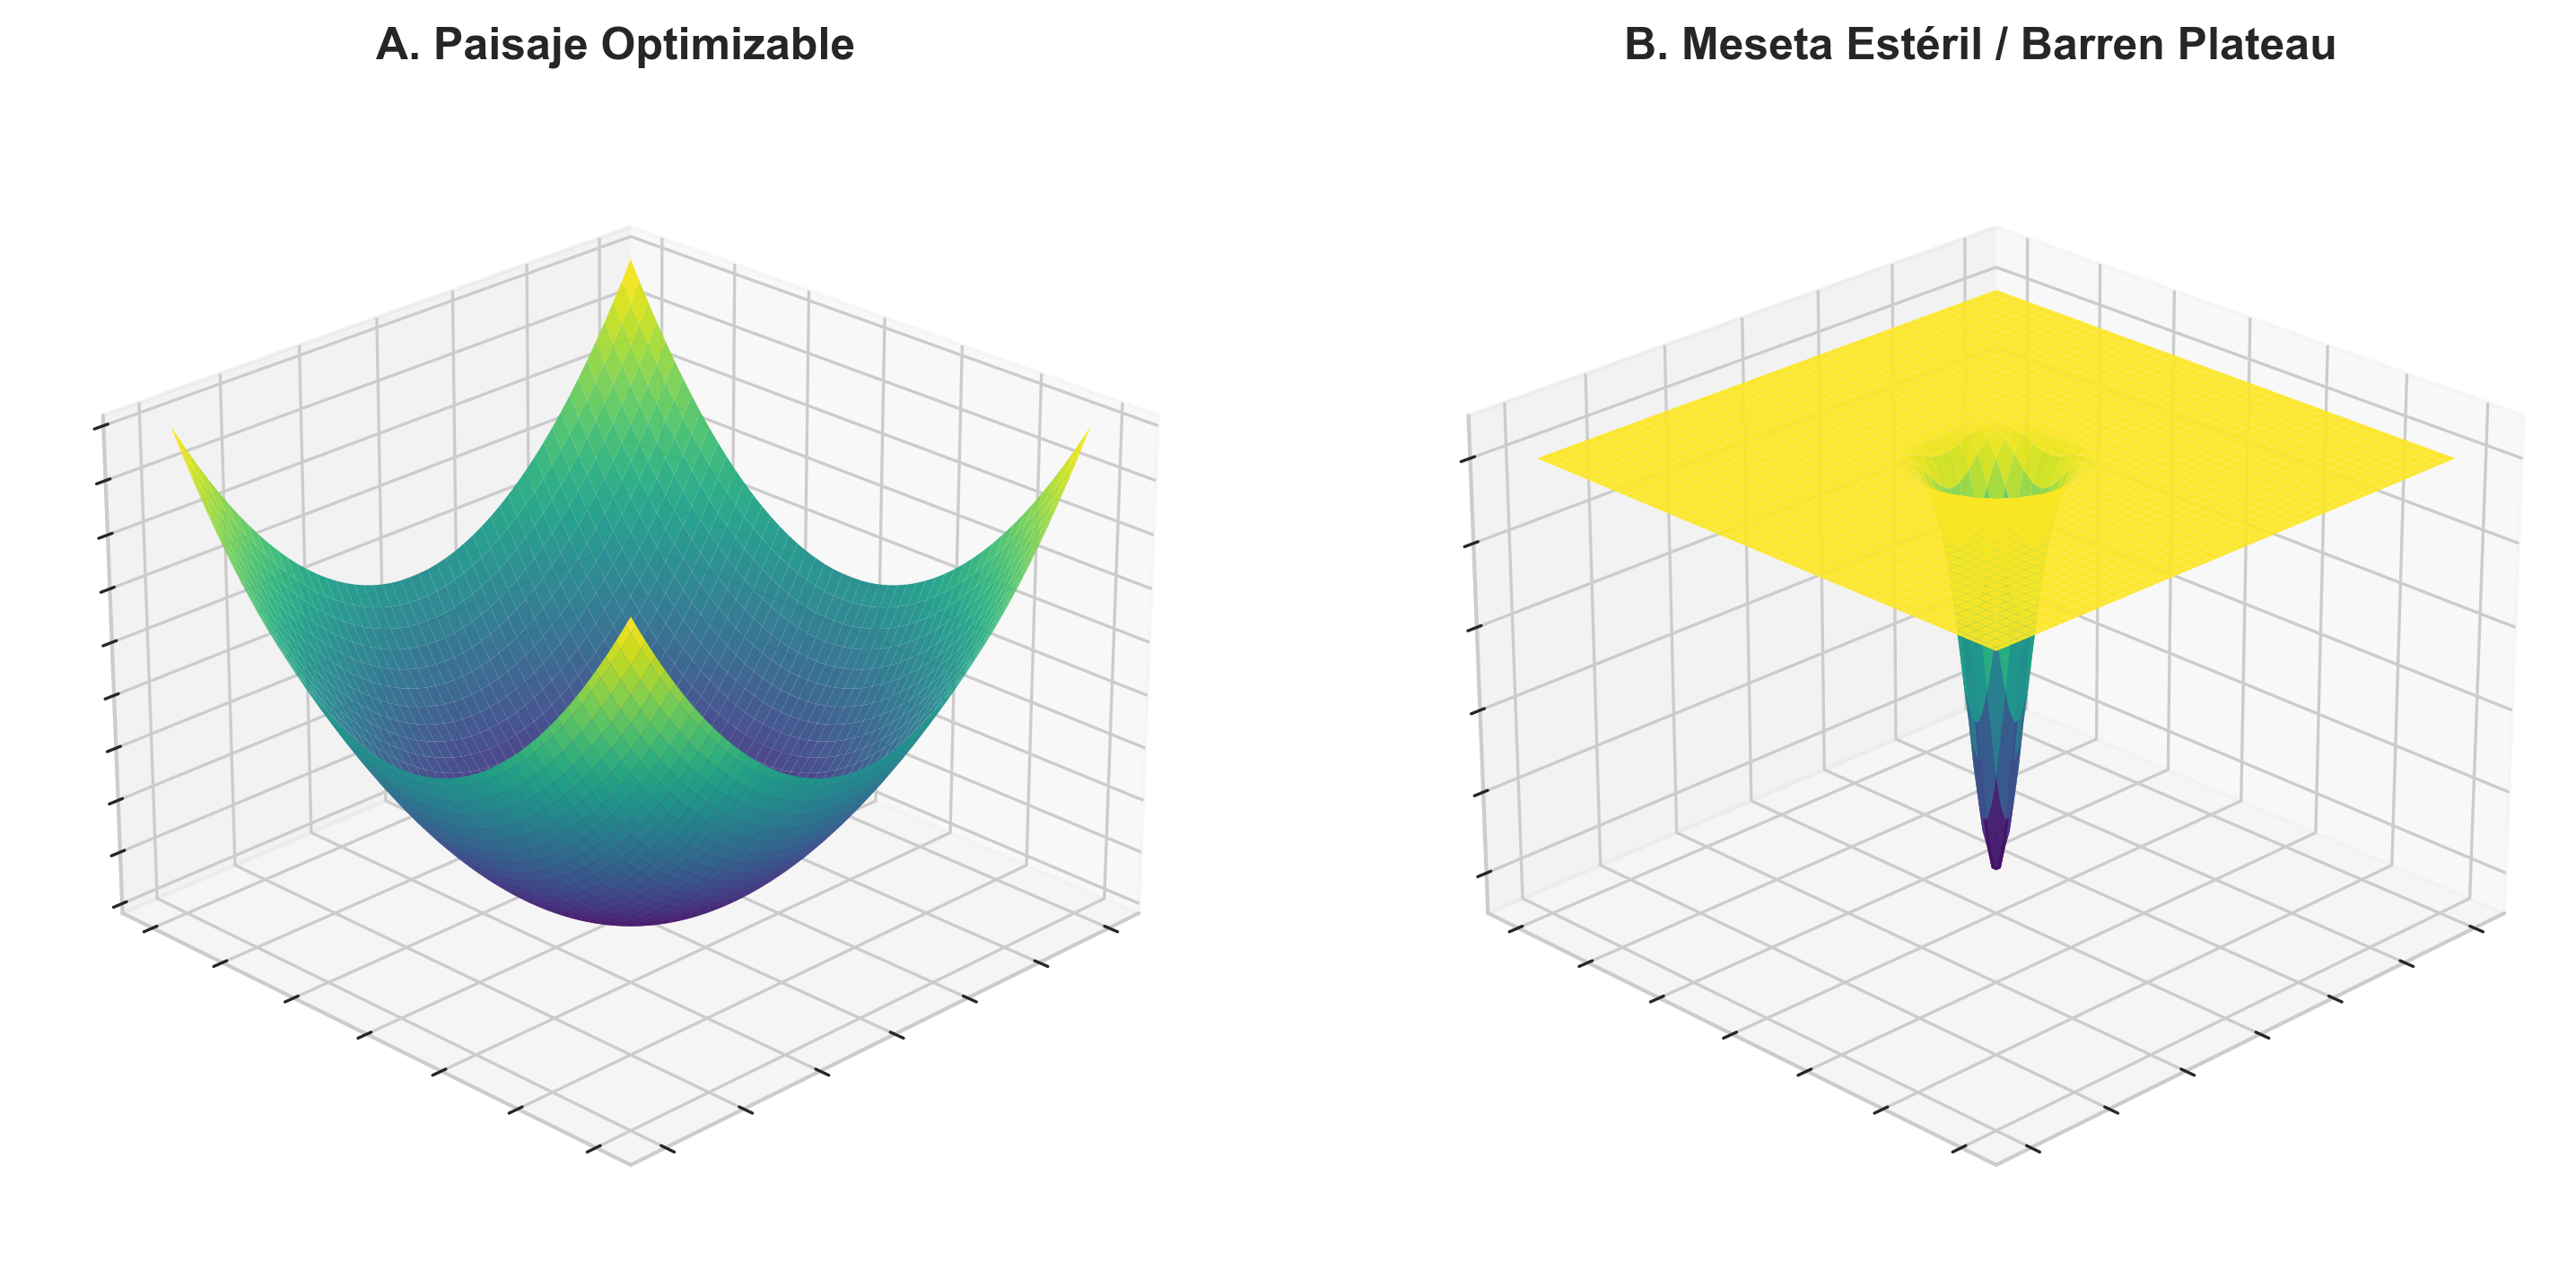
\includegraphics[width=0.95\textwidth]{output/figures/barren_plateaus.png}
    \caption{Representación conceptual del impacto de la varianza del gradiente en algoritmos variacionales. El panel A muestra un paisaje con gradientes fuertes donde un optimizador puede descender fácilmente al mínimo, mientras que el panel B ilustra la meseta estéril (\textit{Barren Plateau}) descrita por McClean \textit{et al.} \cite{McClean2018}, donde el gradiente es cero en casi todo el espacio, impidiendo la convergencia de optimizadores locales clásicos.}
    \label{fig:barren_plateaus}
\end{figure}

\section{Justificación Metodológica y Tecnológica}
\label{sec:justificacion_metodologica}

Para solventar el problema de las mesetas estériles y la ineficiencia asociada a la exploración de estados cuánticos inválidos, la investigación de frontera se orienta hacia el diseño de circuitos con preservación de simetría estructural (\textit{symmetry-preserving ansatzes}) \cite{Barkoutsos2020}. En lugar de penalizar los estados no factibles \textit{a posteriori} de forma matemática, este enfoque rediseña los operadores cuánticos para restringir la dinámica del circuito de forma nativa al subespacio de soluciones válidas.

Para el problema de la cardinalidad exacta $K$, el espacio de Hilbert se inicializa mapeando una superposición uniforme restringida a estados que posean exactamente $K$ cúbits en el estado $|1\rangle$, conocidos como estados de Dicke. Posteriormente, el Hamiltoniano mezclador estándar $H_M = \sum X_i$ se sustituye por un operador mezclador XY basado en interacciones de intercambio de espín:
\begin{equation}
    H_{M}^{XY} = \frac{1}{2} \sum_{\langle i,j \rangle} \left( X_i X_j + Y_i Y_j \right)
\end{equation}
Dado que el operador de intercambio preserva la magnetización total del sistema, es decir, conmuta de forma estricta con el operador de número de partículas ($[H_{M}^{XY}, \sum Z_i] = 0$), el circuito cuántico evoluciona confinándose exclusivamente dentro del subespacio geométrico de Dicke $\binom{N}{K}$ \cite{Barkoutsos2020}. 

La justificación fundamental de la arquitectura implementada en este proyecto radica en la notable optimización del espacio combinatorio explorado. Como se detalla en la Figura \ref{fig:confinamiento_espacio}, la formulación estándar QUBO mapea el problema forzando al hardware a evaluar las dimensiones completas de un espacio de Hilbert de tamaño $2^N$, malgastando recursos cuánticos en estados no factibles. Por el contrario, la preservación de simetría restringe el circuito al tamaño exacto del coeficiente binomial de Dicke:
\begin{equation}
    \text{Dim}_{\text{Dicke}} = \binom{N}{K}
\end{equation}
Esta reducción drástica del espacio de búsqueda aminora la profundidad efectiva necesaria en la QPU, estabiliza el cálculo del gradiente clásico ante la mitigación de los \textit{Barren Plateaus} y maximiza la probabilidad de medir soluciones financieras válidas e inmediatamente operables bajo las restricciones de ruido de los procesadores NISQ. La Tabla \ref{tab:estado_arte} sintetiza las ventajas relativas de esta metodología propuesta frente a los paradigmas tradicionales.

\begin{figure}[htbp]
    \centering
    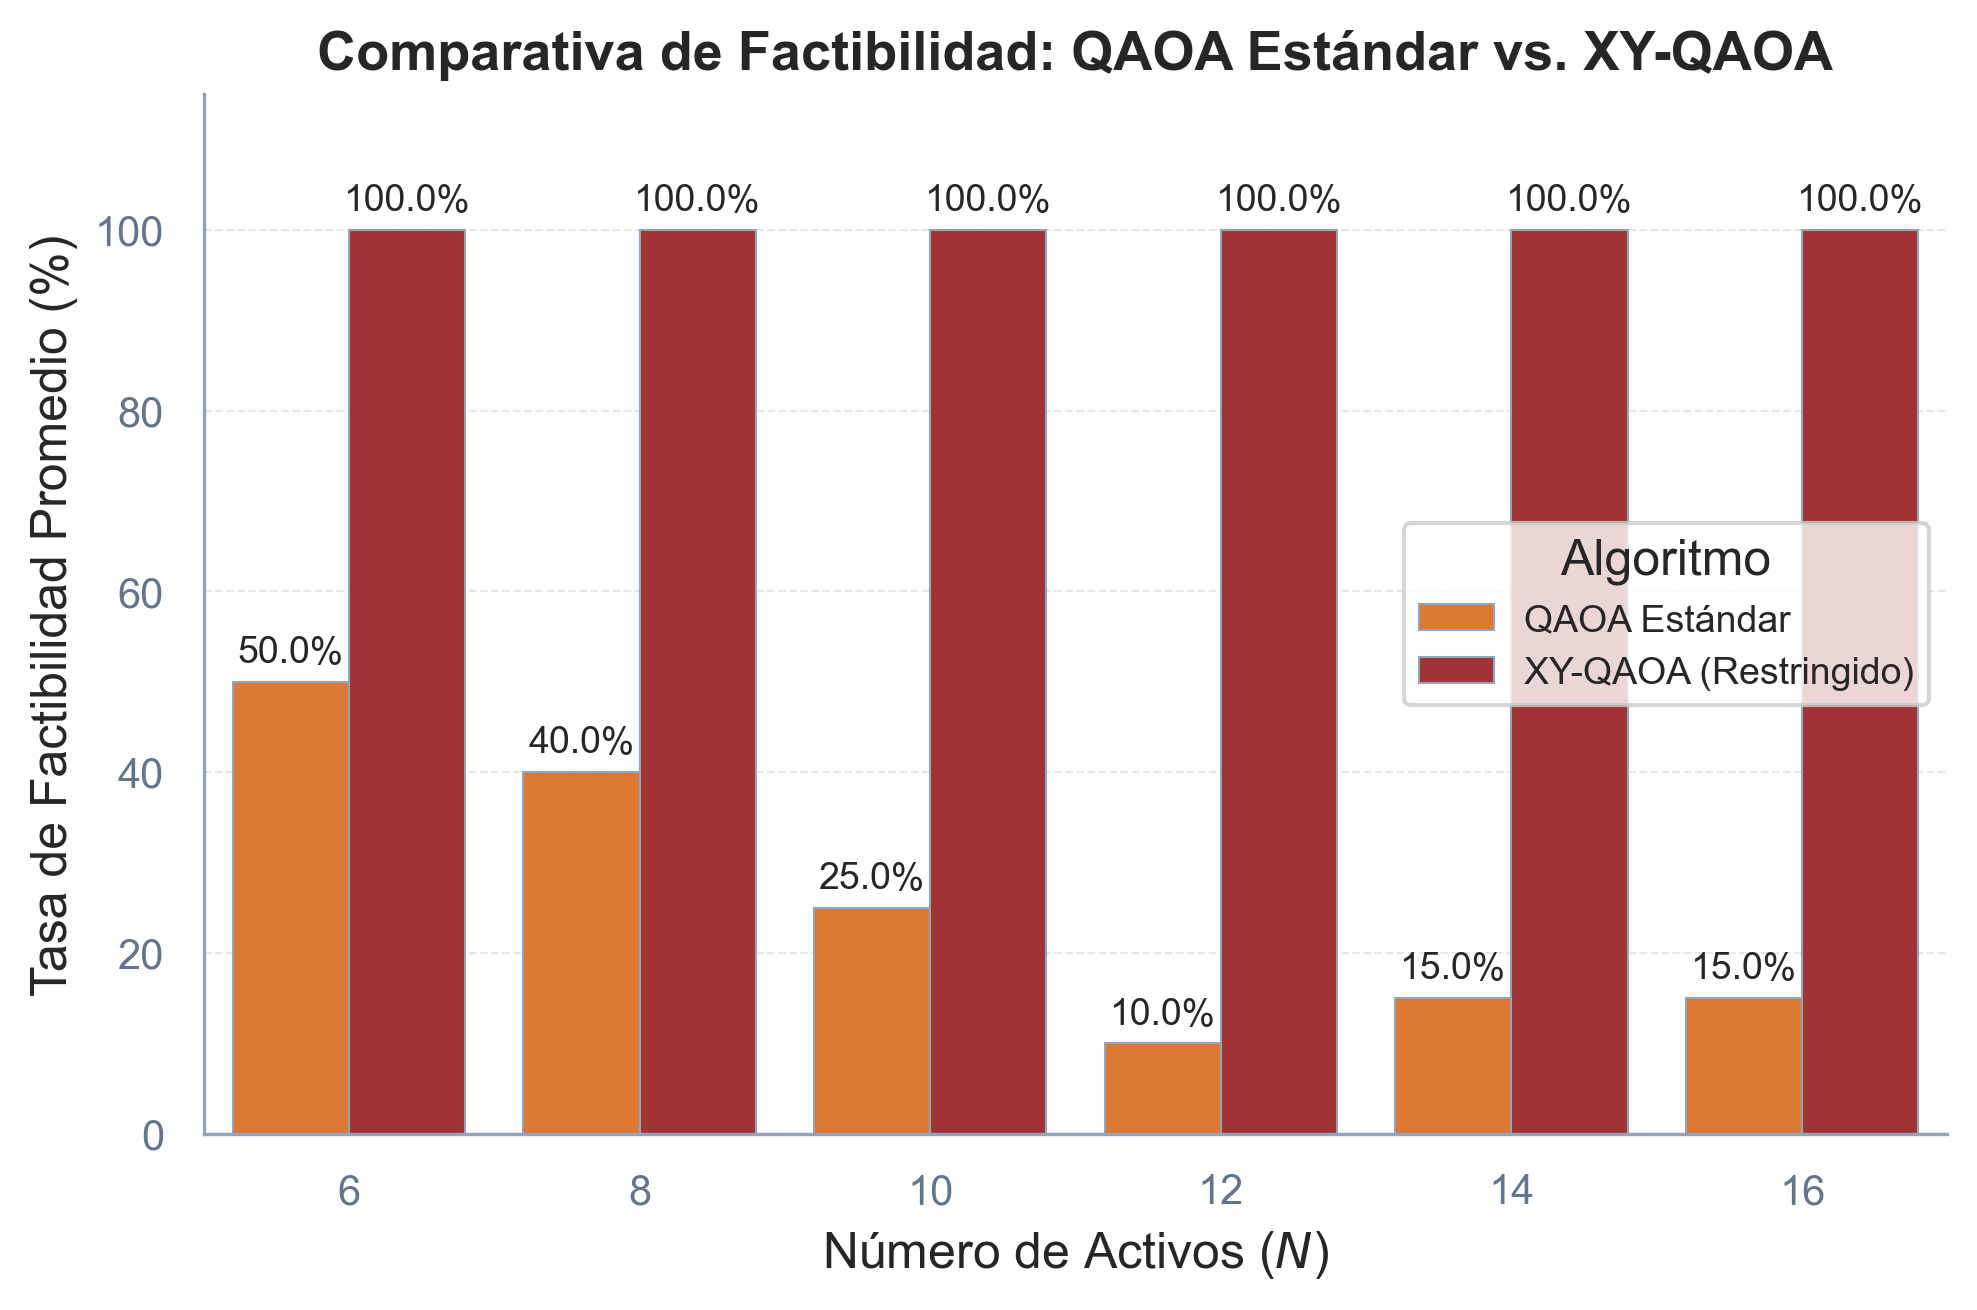
\includegraphics[width=0.85\textwidth]{output/figures/xy_vs_qaoa_feasibility.png}
    \caption{Diferencia conceptual en el espacio de búsqueda. El enfoque QUBO estándar (izquierda) evalúa un espacio abstracto exponencial $2^N$, requiriendo costosas penalizaciones matemáticas. El enfoque de preservación de simetría (derecha) restringe dinámicamente el circuito al subespacio físico de Dicke de tamaño $\binom{N}{K}$, protegiendo la ejecución frente a estados inválidos.}
    \label{fig:confinamiento_espacio}
\end{figure}

\begin{table}[htbp]
    \centering
    \caption{Comparativa taxonómica del estado del arte en algoritmos de optimización combinatoria clásica y cuántica.}
    \label{tab:estado_arte}
    \begin{tabular}{p{2.8cm}p{2.5cm}p{3cm}p{2.2cm}p{2.3cm}}
        \toprule
        \textbf{Algoritmo / Enfoque} & \textbf{Paradigma de Computación} & \textbf{Manejo de Restricciones ($K$)} & \textbf{Eficiencia en Cúbits / Recursos} & \textbf{Escalabilidad en la Era NISQ} \\
        \midrule
        \textbf{Gurobi Optimizer} \cite{Gurobi2025} & Clásico Determinista Exacto & Planos de corte y bifurcación ramificada. & Memoria RAM y CPU escalar exponencial. & Nula para instancias densas ($N \gg 100$). \\
        \addlinespace
        \textbf{Simulated Annealing} & Clásico Estocástico Heurístico & Penalización o rechazo analítico de vecindarios. & Cómputo CPU secuencial ligero. & Alta rapidez temporal, baja garantía de optimalidad global. \\
        \addlinespace
        \textbf{Standard QAOA} \cite{Farhi2014} & Cuántico Basado en Compuertas & Penalización cuadrática en la función de coste. & Requiere $N$ cúbits sin registros auxiliares. & Baja (alto ruido por penalizaciones duras e inestabilidad). \\
        \addlinespace
        \textbf{Quantum Annealing} & Cuántico Adiabático Nativo & Mapeo de penalizaciones QUBO en grafos físicos. & Alta dependencia del grafo de acoplamiento. & Media (afectado por las limitaciones de conectividad de la arquitectura). \\
        \addlinespace
        \textbf{XY-QAOA (Propuesto)} & Cuántico Híbrido Variacional & Confinamiento físico en el subespacio de Dicke. & Optimizado a $N$ cúbits lineales libres de ancillas. & Alta (menor profundidad de circuito y resistencia al ruido \cite{Barkoutsos2020}). \\
        \bottomrule
    \end{tabular}
\end{table}